\subsection{Información personal}

  \subsubsection{Modificar contraseña}\label{modificarPassword}

  \paragraph{}Para este usuario, estará disponible la posibilidad de cambiar su
  contraseña en el sistema. Para llevar a cabo esta operación, deberá rellenar
  el formulario que se muestra en la figura
  \ref{capturaPantallaModificarPassword}.

  \begin{figure}[!ht]
    \begin{center}
      \fbox{
      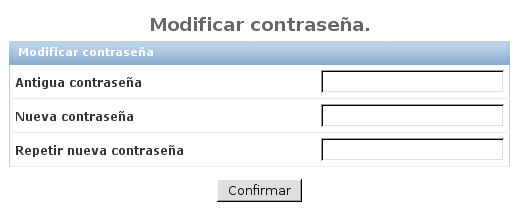
\includegraphics[scale=0.55]{4.Funcionamiento_Aplicacion/4.3.Gestion/4.3.2.Administrador_Centro/4.3.2.9.Informacion_Personal/modificar_password.png}
      }
      \caption{Captura de pantalla del formulario de modificación de la contraseña.}
      \label{capturaPantallaModificarPassword}
    \end{center}
  \end{figure}

  \paragraph{}Una vez rellenado el formulario, se pulsará el botón
  \textit{Confirmar}, el cual se puede ver en la figura
  \ref{capturaBotonConfirmar}. Si el formulario rellenado es válido, y no tiene
  errores, se modificará la contraseña del usuario en el sistema. En caso de
  contener información no válida, como por ejemplo que no coincida la repetición
  de la nueva contraseña, un mensaje de error aparecerá indicando los campos
  del formulario que no han pasado la validación, los cuales habrá que volver
  a introducir para modificar la contraseña del usuario en el sistema.
